\documentclass{beamer}

<<<<<<< Updated upstream
=======
%\usetheme{AnnArbor}
\usetheme{Boadilla}
\usecolortheme{whale}

>>>>>>> Stashed changes
\usepackage[utf8]{inputenc}
\graphicspath{{../Graphics/}}

%Information to be included in the title page:
\title{Heat Energy Sources in Canada}
\author{Noah Bolohan, Anton Iatcenko, Ryan Thiessen, Yakine Bahri, Benjamin MacAdam, Alireza Yazdani}
\institute{Math\textsuperscript{Industry}}

\date{August 2020  \\ \vspace{30pt} 
\includegraphics[scale=0.3]{pims_logo.png} }



\begin{document}

\frame{\titlepage}

\begin{frame}
\frametitle{The Data Set}
what the data is, where it came from
\end{frame}


\begin{frame}
\frametitle{Primary heating types in Canada: 2013-2017}
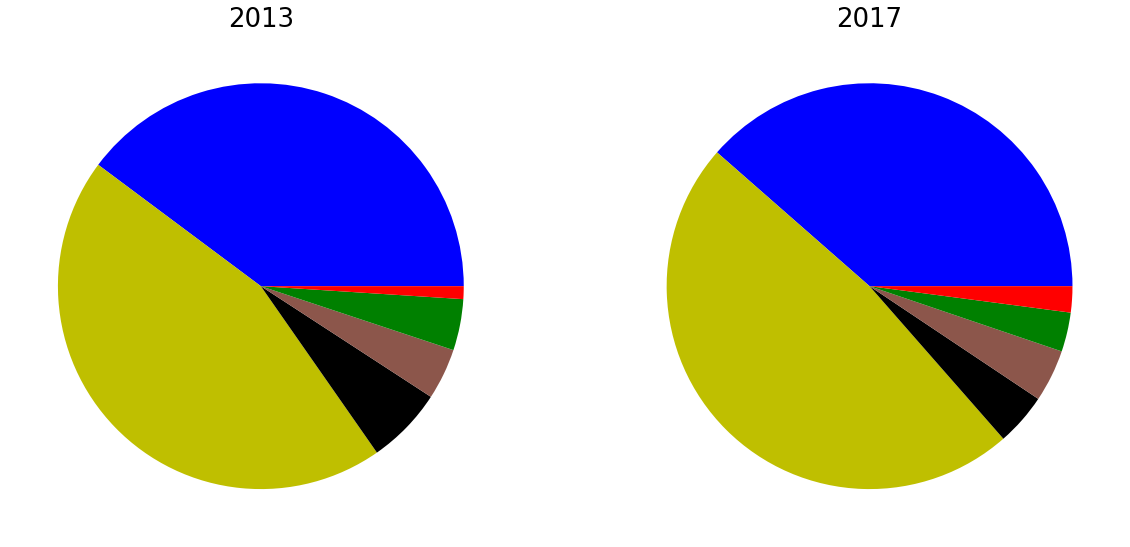
\includegraphics[width=\textwidth]{Canada20132017.png}
\end{frame}


\begin{frame}
\frametitle{Change Over Time I}
stacked bars (4 per slide)
\end{frame}


\begin{frame}
\frametitle{Change Over Time II}
stacked bars (4 per slide)
\end{frame}


\begin{frame}
\frametitle{Change Over Time III}
stacked bars (4 per slide)
\end{frame}


\begin{frame}
\frametitle{Province Groupings}
stacked bars (all together)
\end{frame}


\begin{frame}
\frametitle{Cause of the Groupings: Natural Gas}

\end{frame}


\begin{frame}
\frametitle{Cause of the Groupings: Electricity}

\end{frame}


\begin{frame}
\frametitle{Cause of the Groupings: Atlantic Provinces}

\end{frame}



\begin{frame}
\frametitle{Summary}

No change over time. 

The dependence is predominantly geographic. 

Thanks for your attention.  

\end{frame}













\end{document}



















